\chapter{Implementation}
\label{cha:Implementation}

In this chapter the most important details about the implementation are revealed. The general idea behind the workflow is described and presented in the form of sequence diagrams. Class and package diagrams show basic architecture of the implementation, and the most important structures are discussed with a few interesting source code listings.

\section{Packages}
As could be seen in the previous section, whole plugin is divided into three main parts: plugin management, speech recognition and interpretation. Classes important for each particular part are placed in the respective packages. The package structure can be seen in Fig. \ref{fig:packageDiagram}. 

\begin{figure}[hbt!]
    \centering
    \fbox{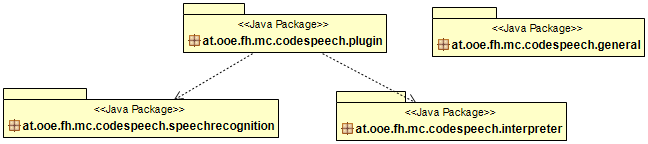
\includegraphics[width=0.9\textwidth]{images/PackageDiagram.png}}
    \caption{Basic package structure and dependencies.}
    \label{fig:packageDiagram}
\end{figure}

\subsection{\textit{general} package}
The \textit{general} package contains elements of the system that are common for every other package. Its subpackage \textit{exceptions} is a place for classes that can be used to throw exceptions. As for now there exist two of those, namely \texttt{NotImplementedException} and \texttt{InvalidNumberException}. The \textit{events} subpackage consists of \texttt{Even<T>} abstract class that is a parent of any other implementation of an event to be handled by \texttt{EventHandler}. An example of a child event is \texttt{OnInterpretationFinishedEvent} of \textit{interpreter} package. Finally, \textit{utils} subpackage has two static utility classes that allow operations on strings (\texttt{StringUtils}) and conversion of word to number (\texttt{WordToNumber}).


\subsection{\textit{plugin} package}
The \textit{plugin} package consists of elements that are related to the management of a plugin. It contains the most important \texttt{PluginManager} class, as well as static helper classes used for handling of operations performed on text editors, package explorer, abstract syntax tree and for global search functionality. These static classes are named \texttt{EditorManager}, \texttt{PackageExplorerManager}, \texttt{ASTManager} and \texttt{Searcher} respectively and are held in \textit{utils} subpackage. Another class contained in \textit{plugin} package is \texttt{ToggleSpeechRecognition-} \texttt{Handler}, which turns on or off active listening when menu button is toggled. For debugging purposes an additional dialog box was added to the IDE, which allows to skip speech recognition part and enter the command in the text form. The dialog is implemented as \texttt{CommandDialog}. By pressing the OK button an \texttt{EnterCommandHandler} is triggered. All three of these are part of the plugin and therefore they can also be found in the subpackage \textit{menu}.

\subsection{\textit{speechrecognition} package}
As the name suggests this package holds implementation of speech recognition elements. The most important one is \texttt{SpeechRecognizer} abstract class, which enables usage of many different SR toolkits. Currently there are three different classes utilizing different APIs that inherit from it, namely \texttt{Sphinx4SpeechRecognizer}, \texttt{PocketsphinxSpeechRe-} \texttt{cognizer} and \texttt{GoogleSpeechRecognizer}. These were put into subpackages \textit{cmusphinx} and \textit{googlespeech}. To change between SR technologies a specific \texttt{Enum} value of \texttt{SREngine-} \texttt{Type} has to be passed into the \texttt{SpeechRecognitionFactory}. The factory initializes and returns specified \texttt{SpeechRecognizer} object. Selection of SR toolkit is not available from the user side, by default \texttt{GoogleSpeechRecognizer} is returned.  \texttt{SpeechRecognitionLi-} \texttt{stener} interface which provides handling methods for recognition events is also present in this package, together with the event classes. These children of \texttt{Event<T>} class are found in \textit{events}. \texttt{Microphone} class is used for management of audio recording, therefore is a part of this package.

\subsection{\textit{interpreter} package}
The main classes of this package are \texttt{Interpreter}, \texttt{InterpreterContext} and \texttt{Command}. \texttt{InterpreterListener}, which provides a way to handle interpretation events can also be found in here. For now only one such event exists, namely \texttt{OnInterpretatioFinished-} \texttt{Event} placed inside \textit{events} subpackage. The \textit{grammar} subpackage is where ANTLR generated classes are being kept. Every keyword listener that extends \texttt{BaseKeywordListener} (including \texttt{BaseKeywordListener} itself) has been placed in \textit{listeners} subpackage. \texttt{Opera-} \texttt{tion} interface together with its implementations can be found in \textit{operations}. They provide methods that consist of logic for performing specific actions, such as creation of a structure, navigation \etc Therefore, according to usage they have been separated into three categories that exist so far: \textit{creation}, \textit{modification} and \textit{navigation}. In order to ensure creation/modification of a proper programming structures, their representation has been introduced in a form of models. They all extend \texttt{Model} abstract class and can be found \textit{models} subpackage. Examples of such models are \eg \texttt{ClassModel}, \texttt{MethodInvocationModel} or \texttt{ConditionalModel}.


\section{Most important classes and interfaces}

In Fig. \ref{fig:classDiagram} one can find class diagram presenting the most important classes together with their relations. Many of these classes rely on other ones that are not depicted in here to ensure readability of the graph. Some of them will be mentioned, described or presented on another images further on. In the center of the graph with yellow color there is \texttt{PluginManager}. On its left side, depicted in green there are classes responsible for interpretation and on the right with blue color, those that take care of speech recognition. For the sake of simplicity only one subclass of \texttt{BaseListener}, \texttt{Model} and one implementation \texttt{Operation} are depicted. It is to show an example of how these classes are related. The relationships of other children are analogous.

\begin{sidewaysfigure}
    \centering
    \fbox{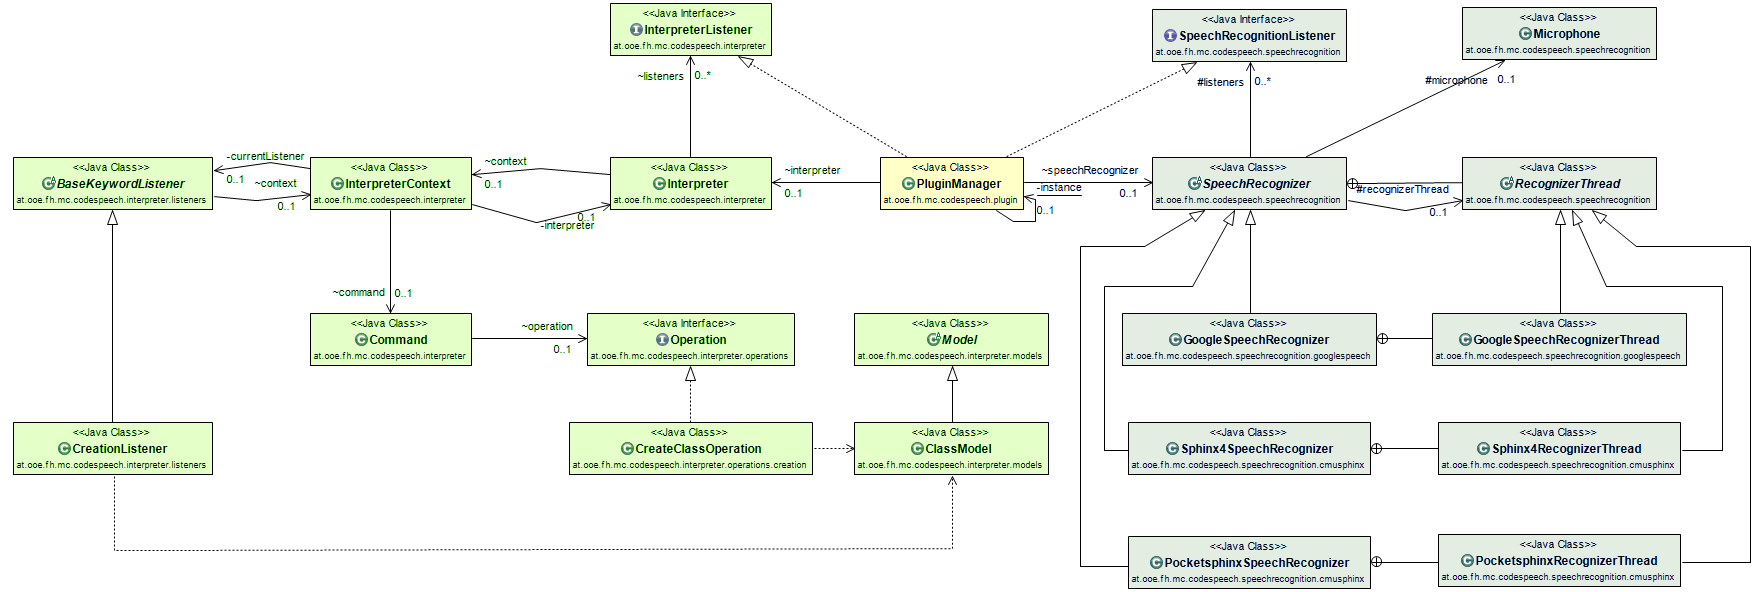
\includegraphics[width=\textwidth]{images/ClassDiagram.png}}
     \caption{Class diagram representing the most important classes and their relations.}
    \label{fig:classDiagram}
 \end{sidewaysfigure}


\subsection{PluginManager}

\texttt{PluginManager} is the heart of the plugin (usually called ``Activator'' in official documentation of PDE development). It extends \texttt{Plugin} class, which is a part of OSGi framework. Its \texttt{start} method is called the first time the plugin is initialized, which happens whenever any element of plugin is required for the first time. It is there, where all necessary objects are created. Additionally, \texttt{PluginManager} implements two interfaces created by the author, namely \texttt{SpeechRecognitionListener} and \texttt{InterpreterListener}. As the names suggest, these are the interfaces that allow handling of events related to recognition of speech and text interpretation respectively. During initialization of the plugin \texttt{Interpreter}, as well as a \texttt{SpeechRecognizer} is created. \texttt{PluginManager} also implements \texttt{IPartListener2} in order to get notified in case of any change in text editors. So far this is utilized only to keep track of currently opened editor.

\subsection{SpeechRecognizer}
\texttt{SpeechRecognizer} is an abstract class and a parent of \texttt{Sphinx4SpeechRecognizer}, \texttt{PocketsphinxSpeechRecognizer} and \texttt{GoogleSpeechRecognizer} which utilize different SR toolkits. It contains \texttt{Microphone}, \texttt{EventHandler}, \texttt{Mode} and \texttt{RecognierThread} instances, and also a list of \texttt{SpeechRecognitionListeners}. It provides methods to start and stop audio listening. As it is implemented now, three modes of recognition are possible: continuous speech, based on grammar and based on keyphrases. Only CMUSphinx recognizers provide a way for grammar-based recognition, and only PocketSphinx API can recognize in keyphrase mode. Implementation uses only continuous speech as for now. If any new SR toolkit is to be used, simply a new class has to inherit \texttt{SpeechRecognizer} and use its API in there. 
\texttt{Microphone} is responsible for gathering audio data, \texttt{Mode} is an enumeration type and its instance helps to keep track of current recognition mode.

\subsection{RecognizerThread}
\texttt{SpeechRecognizer's} inner class \texttt{RecognizerThread} extends \texttt{Thread} and it is in its \texttt{run} method where the main process of recognition is performed. This class has to be extended as well when new SR toolkit is being implemented. The most important to override are three methods: \texttt{beforeRecognition}, \texttt{recognize} and \texttt{afterRecognition}. Starting from the beginning, \texttt{beforeRecognition} is where all operations that are mandatory just before the recognition are performed. In \texttt{recognize} method the actual recognition logic is done. Finally, \texttt{afterRecognition} is where all of the post recognition operations, such as changing state to finished or breaking a connection need to be placed to avoid problems in future recognition.

\subsection{Interpreter}
Next on the list is the \texttt{Interpreter} class. It contains \texttt{InterpreterContext}, \texttt{EventHan-} \texttt{dler} and a list of \texttt{InterpreterListener} instances. Its main functionality is in \texttt{inter-} \texttt{preter} method, which is being called upon when the recognition is done. It receives a text in a form of \texttt{String}. If the text is not empty, everything needed for parsing is set up, together with generated by ANTLR tool \texttt{GrammarParser} and \texttt{GrammarLexer}. Once everything is ready, \texttt{ParseTreeWalker} walks through a tokenized tree. Details are shown in Program \ref{list:interpretation}. Once \texttt{finish} method is called by the context, \texttt{OnInterpretationFi-} \texttt{nishedEvent} is posted.

\begin{program}[hbt!]
    \caption{Start of interpretation procedure.}
    \label{list:interpretation}
    \begin{JavaCode}
public void interpret(String utterance) {
	if(!utterance.isEmpty()) {			
		GrammarLexer lexer = new GrammarLexer(CharStreams.fromString(utterance));

		CommonTokenStream tokens = new CommonTokenStream(lexer);
		GrammarParser parser = new GrammarParser(tokens);

		ParseTreeWalker walker = new ParseTreeWalker();
		
		walker.walk(context.getCurrentListener(), parser.command());	
	}
}    \end{JavaCode}
\end{program}

\subsection{InterpreterContext}
This class was created to gather all important data throughout the process of interpretation. Its instance is passed between listeners when they change. It contains many fields such as \texttt{boolean isAbstract} or \texttt{String simpleType} that are being set when a keyword, such as ``abstract'' or ``simpleType'' respectively, was detected and the corresponding method of a listener called. Once it is known what operation is to be performed and which of these properties are important, proper object is created using these properties. Additionally \texttt{InterpreterContext} contains of \texttt{Command} object, which at the proper moment is set and at the end of interpretation process passed as an argument to the listeners by the event handler.

\subsection{BaseKeywordListener}
Inheriting from ANTLR generated \texttt{GrammarBaseListener}, \texttt{BaseKeywordListener} is an abstract parent of every other listener to be used for grammar analysis of the command. It provides common functionality for other listeners like building up \texttt{Command}, canceling if something went wrong (going back to initial state) or finalizing the process. It provides an opportunity of overriding any method that is triggered when a specific token is entered or exited. An example of such method is depicted in Program \ref{list:enterPackageKeyword}. It shows a method of \texttt{SelectionListener} activated after the keyword ``select'' was detected. Once keyword ``package'' is found, \texttt{enterPackageKeyword} method of this listener is triggered and a proper model together with operation is set up.

\begin{program}[hbt!]
    \caption{Entering ``packageKeyword'' token in \texttt{SelectionListener}.}
    \label{list:enterPackageKeyword}
    \begin{JavaCode}
@Override
	public void enterPackageKeyword(PackageKeywordContext ctx) {
		super.enterPackageKeyword(ctx);

		changeProperty(new PackageModel());
		changeOperation(new SelectPackageOperation());
	}    \end{JavaCode}
\end{program}

\subsection{Command}
\texttt{Command} is a simple but important class. It has two objects that are being set during the interpretation. First one is an instance of \texttt{Operation} and the second is \texttt{Object property}. When the command is executed, \texttt{perform} method of operation is called with the \texttt{property} object passed as argument.

\subsection{Operations}
\texttt{Operation} is an interface and each class that agrees to fulfill its contract has to implement \texttt{perform} method. Each operation is different, therefore each is implemented separately. Examples of operations are \eg \texttt{CreateClassOperation} or \texttt{ChangeReturnType-} \texttt{Operation} or \texttt{SelectAndOpenClassFileOperation}. An example of yet another operation is given in Program \ref{list:operationExample}.


\begin{program}[hbt!]
    \caption{\texttt{AddArgumentOperation} class. It can be seen that operation classes contain of only one method and nothing else. Operations use utility methods provided by \texttt{ASTManager} to perform changes to AST and by \texttt{EditorManager} to update compilation unit and place cursor into the new position.}
    \label{list:operationExample}
    \begin{JavaCode}
public class AddArgumentOperation implements Operation {

	@Override
	public void perform(Object property) throws Exception {
		if(property instanceof String) {
			ASTNode node = ASTManager.getNextNodeOfType(
		    	ASTManager.currentNode, MethodInvocation.class);
			if (node != null && node instanceof MethodInvocation) {
				AST ast = node.getAST();
				ASTRewrite rewriter = ASTRewrite.create(ast);
				ListRewrite listRewrite = rewriter.getListRewrite(
				    node, MethodInvocation.ARGUMENTS_PROPERTY);
				
				MethodInvocation methodInvocation = (MethodInvocation) node;
				SimpleName name = ast.newSimpleName((String) property);
				listRewrite.insertLast(name,  null);
			
				EditorManager.updateCompilationUnit(rewriter.rewriteAST());
				EditorManager.moveToNode(name);		
			}
				
		}
	}
}   \end{JavaCode}
\end{program}

\subsection{Models}
As mentioned before, in order to create a proper structure with correct properties models were introduced. Each model is different, depending on which AST node or program structure it represents. All models inherit a getter and setter of a \texttt{String phrase}. The reason for that is to avoid huge switch statement and to set names of certain structures, set conditions into others \etc in a unified way.

\section{Workflow}

Below, the most important parts of the working cycle are presented and described in detail. The first important part of a workflow is speech recognition, the second is interpretation. For better understanding of the activities, each of them is depicted in the form of sequence diagrams. Implementation of the most important part of speech recognition is also enlisted.

\subsection{Speech recognition}

In Fig. \ref{fig:sequenceRecognition} a sequence diagram presenting speech recognition process is shown. Once plugin is turned on (via toggle of menu button) speech recognition class starts its recognition thread. At the beginning microphone recording is started and \texttt{beforeRecognition} method called. Afterwards, functionality loops until it is interrupted. The first thing inside the loop is a check for timeout. If it did occur, an \texttt{OnTimeoutEvent} is send, if not, an input stream of a \texttt{Microphone} object is read. If audio was successfully read, \texttt{recognize} method is called. At the end of successful recognition \texttt{OnResultEvent} should be posted. The main loop is surrounded by try-catch-finally block to catch any occurring exceptions that might be thrown in the process and to ensure that \texttt{afterRecognition} is called even if something went wrong. At the end microphone has to stop its recording. The full implementation of the process can be found in Program \ref{list:recognitionRun}.

\begin{program}[hbt!]
    \caption{RecognizerThread's run method.}
    \label{list:recognitionRun}
    \begin{JavaCode}
    @Override
    	public void run() {
    		long startTime;
    		long elapsedTime;
    
    		microphone.startRecording();
    
    		beforeRecognition();
    
    		startTime = System.currentTimeMillis();
    
    		try {
    			while(!interrupted) {	
    				elapsedTime = System.currentTimeMillis() - startTime;
    
    				if(timeOut(elapsedTime)) {
    					eventHandler.post(new OnTimeoutEvent(listeners));
    					break;
    				}		
    
    				byte[] bytes = new byte[BUFFER_SIZE];
    				int numberOfBytes = microphone.getStream().read(bytes);
    
    				if(numberOfBytes > 0) {					
    					recognize(bytes, numberOfBytes);
    					startTime = System.currentTimeMillis();
    				}
    			}
    		} catch (Exception exception) {
    			exception.printStackTrace();
    		} finally {
    			afterRecognition();
    			microphone.stopRecording();	
    		}
    
    	}    \end{JavaCode}
\end{program}

\begin{sidewaysfigure}
    \centering
    \fbox{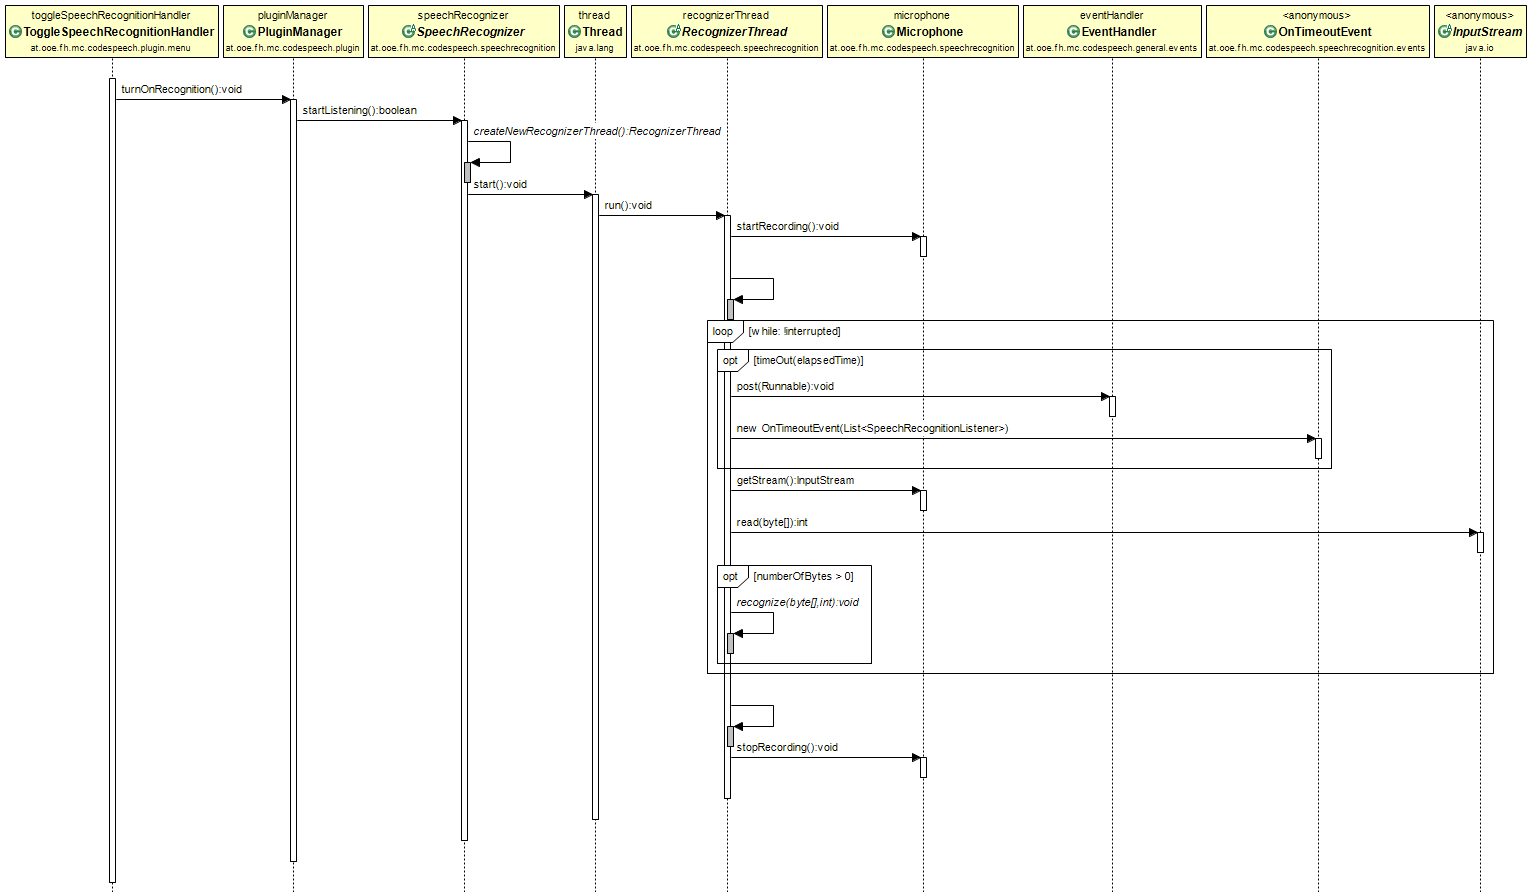
\includegraphics[width=\textwidth]{images/SequenceRecognition.png}}
    \caption{Sequence diagram showing process from start to speech recognition.}
    \label{fig:sequenceRecognition}
\end{sidewaysfigure}

\subsection{Interpretation}

Once the sentence is recognized, an \texttt{OnResultEvent} event is triggered and the utterance is sent to all listeners. The main one is \texttt{PluginManager} class, which delegates recognized text to \texttt{Interpreter}. An example of interpretation procedure is depicted as sequence diagram in Fig. \ref{fig:sequenceInterpretation}. Once \texttt{interpret} method of \texttt{Interpreter} object is called, it initializes all the necessary objects needed for ANTLR parsing and starts walking through the parsed tokens. Interpretation always starts with an \texttt{InitialListener} (all listeners extend \texttt{BaseKeywordListener}), which first listens to the keyword determining operation type and then delegating parsing to another listener accordingly. Listeners can be viewed as the state, which provides different functionality depending on the current situation. Once the listener is changed the interpretation continues. During the whole process, \texttt{InterpreterContext} object is being built up, together with its \texttt{Command} object. Once the whole text has been analysed, an \texttt{OnInterprataionFinished} event is triggered and \texttt{InterpreterListeners} are notified. Here again, \texttt{PluginManager} is a main subscriber. Once receiving a notification, \texttt{PluginManager} performs specific action using generated \texttt{Command}.

\begin{sidewaysfigure}
    \centering
    \fbox{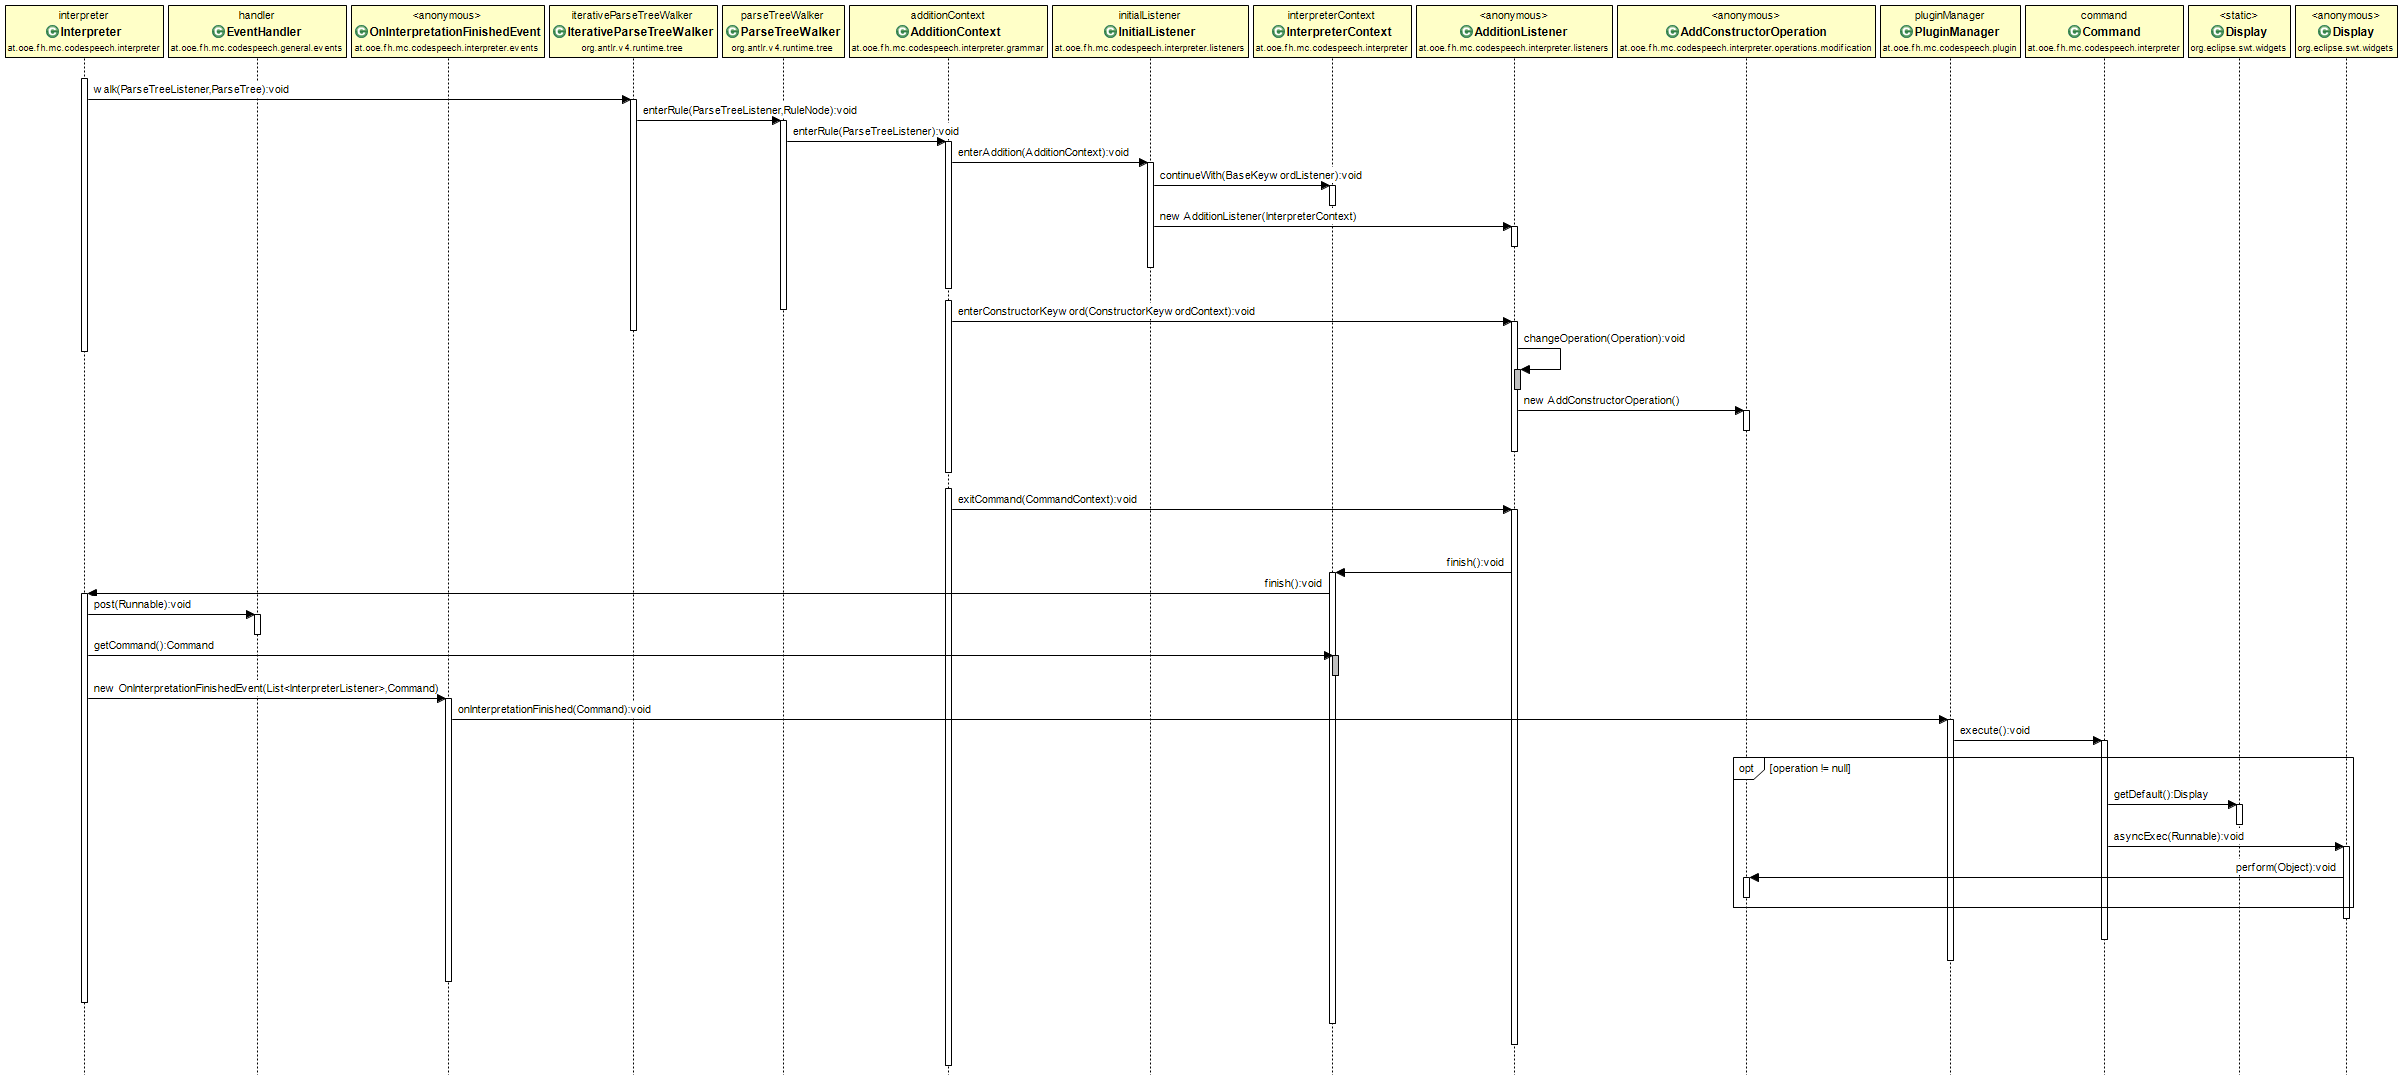
\includegraphics[angle=180,width=\textwidth]{images/SequenceInterpretation.png}}
    \caption{Sequence diagram showing interpretation from start of walking through parsed text to execution of operation.}
    \label{fig:sequenceInterpretation}
\end{sidewaysfigure}

\subsection{Performing operation}

Operations have different responsibilities depending on action they need to execute. Some modify AST by adding new node, deleting or changing one, others select an element in the package explorer or navigate in the currently open editor. In order to perform its task on IDE \texttt{Operation} has to use Eclipse API. Some common functionality has been derived and placed into utilization classes such as \texttt{EditorManager}, \texttt{ASTManager} and \texttt{PackageExplorerManager}. In Fig. \ref{fig:sequenceOperation} a sequence diagram showing the workflow of inserting new \textit{if statement} is shown as an example.

\begin{sidewaysfigure}
    \centering
    \fbox{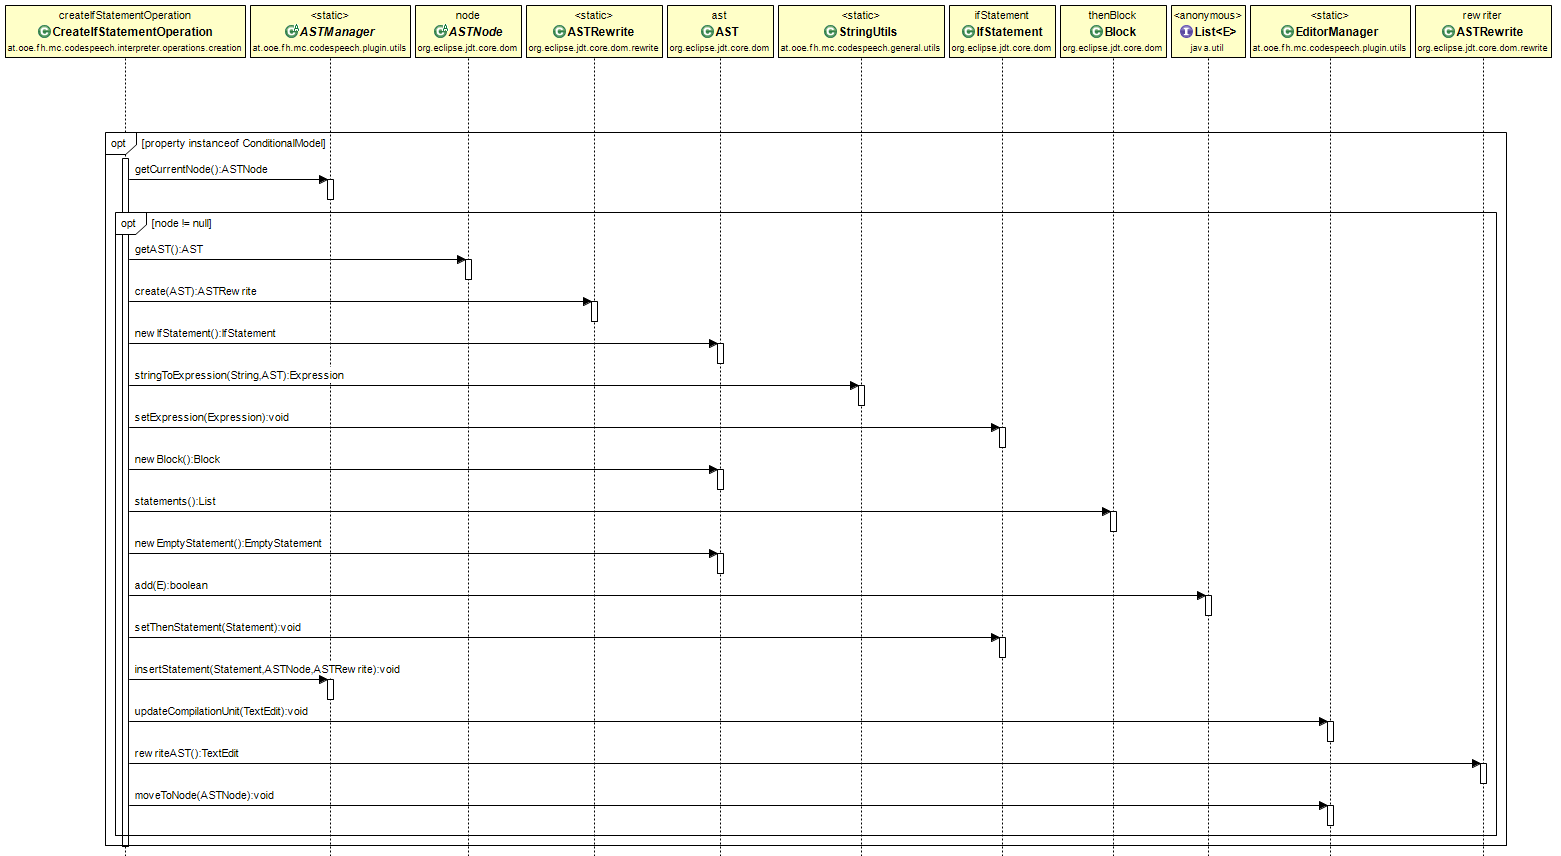
\includegraphics[width=\textwidth]{images/SequenceOperation.png}}
    \caption{An example of operation workflow for operation modifying AST. The use of utilization static classes such as \texttt{StringUtils}, \texttt{ASTManager} and \texttt{EditorManager}.}
    \label{fig:sequenceOperation}
\end{sidewaysfigure}

\section{Implemented features}
At the current state CodeSpeech provides a limited amount of functionalities. In this section their a complete list can be found. Features have been divided into three groups: creation, modification and navigation and they are presented in Tab. \ref{tab:creationFeatures}, Tab. \ref{tab:modificationFeatures} and Tab. \ref{tab:navigationFeatures} respectively. Some of the most interesting features are described in more detail in the following subsections.

\subsection{Error Correction}
Currently the only error correction measure that works is inside the text editor. Since programming is mostly happening in it, it therefore covers most of the cases. By giving the command ``undo last'' the last performed action will be reversed. It can come in handy at times, because the alternative is to delete the whole structure and create it anew. This of course would add to delay and frustration of the user. Unfortunately, when a wrong element is created in the package explorer, such as a project, package or a compilation unit with wrong name it has to be removed and the process repeated.

\subsection{Free Speech Mode}

Unfortunately, because of time limits the current state of the project does not allow for creation of the whole program from scratch. In some cases the use of mouse and keyboard is inevitable. In order to limit this need to the absolute minimum, a special free speech mode was added to the implementation. This mode is the latest addition and is entirely experimental. It allows to enter text as it is recognized, with a small modifications to the text, such as changing it to lower case and removing the spaces between words separated by periods (which is supposed to make up for the lack of nested OOP calls, such as \texttt{System.out.println()}). This mode could be turned on via ``enter free speech'' command, and analogically, exited by saying ``exit free speech''. To ensure easy error correction in case of wrong recognition, a possibility to reverse last change was kept for this mode.

\section{Addition of new functionality}

Once the design of the basic structure was established, adding new functionalities became quite easy. An example will be given on one of the latest features added into the program, which allows entering text straight into the editor. 

Basically whenever a new feature is to be implemented, what has to be done first is the addition of a new parser rule, with which the action is to be called, to the grammar. Fig. \ref{fig:grammarChange} depicts newly inserted phrases. When modification is done and the grammar is ready, ANTLR files have to be generated as described in the official documentation (or in \textit{Tools} chapter). 

\begin{figure}[hbt!]
    \centering
    \fbox{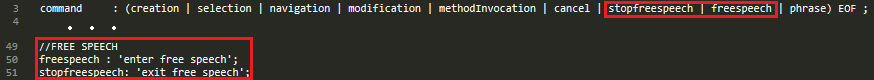
\includegraphics[width=1\textwidth, angle=0]{images/AddingNewPhrase.png}}
    \caption{Part of grammar. The text in red frame has been added to provide new commands.}
    \label{fig:grammarChange}
\end{figure}

For every new parser rule added, the generated files provide new methods for entering and exiting the rule during parsing. In this example such methods are \texttt{enterFreespeech}, \texttt{exitFreespeech},  \texttt{enterStopfreespeech} and \texttt{exitStopfreespeech}. These are inserted into \texttt{GrammarListener} interface and will become available to every other custom listener that implements it (in the current implementation all listeners do through the inheritance of \texttt{BaseKeywordListener}). Whenever it is necessary, a new listener ought to be created. This step can be skipped if one of the existing listeners can be used, \eg if creation of new structure is to be added, an already existing \texttt{CreationListener} will most likely be extended. That is not the case now and so \texttt{FreeSpeechListener} must be created. It is supposed to be activated on \texttt{enterFreespeech}, so this method is overridden in the \texttt{InitialListener}. In there the current listener (state) of the \texttt{InterpreterContext} is changed to the new one like shown in Program \ref{list:enterFreeShpeech}. 

\begin{program}[hbt!]
    \caption{Replacing the current listener to \texttt{FreeSpeechListener} triggered by ``enter free speech'' command.}
    \label{list:enterFreeShpeech}
    \begin{JavaCode}
	@Override
	public void enterFreespeech(FreespeechContext ctx) {
		super.enterFreespeech(ctx);
		context.continueWith(new FreeSpeechListener(context));
	}   \end{JavaCode}
\end{program}

\texttt{FreeSpeechListener} needs to do three things: put text into the editor, be able to reverse changes and go back to the initial state. Adding new text to the editor is new functionality, therefore a new \texttt{Operation} is required. This operation should take raw text as an input, rework it and add it to the editor. The resulting \texttt{FreeSpeechOperation} can be seen in Program \ref{list:freeSpeechOperation}. 

\begin{program}[hbt!]
    \caption{Implementation of new functionality, which works on string and puts it into the current line in the editor.}
    \label{list:freeSpeechOperation}
    \begin{JavaCode}
public class FreeSpeechOperation implements Operation {
	@Override
	public void perform(Object property) throws Exception {
		if(property instanceof String) {
		    EditorManager.enterText(((String) property).replace(". ", "."));
		}
	}
}  \end{JavaCode}
\end{program}

The next feature available from this state is change reversal. The \texttt{UndoOperation} already exists and is simply be reused. Finally, on command ``exit free speech'' the state is changed to the initial one (meaning changing the current listener to \texttt{InitialListener}). Property and operation are cleared. Whole \texttt{FreeSpeechListener} can be seen in Program \ref{list:freeSpeechListener}. That concludes the process of adding new functionality. Details might vary depending on how complex is the command, how many parser rules it consists and so on. Sometimes using more than one listener might be a viable solution to perform a task. 
\begin{program} [hbt!]
    \caption{Implementation of free speech state that is being triggered by three different commands.}
    \label{list:freeSpeechListener}
    \begin{JavaCode}
public class FreeSpeechListener extends BaseKeywordListener {
    ...
	@Override
	public void enterPhrase(PhraseContext ctx) {
		super.enterPhrase(ctx);
		changeProperty(ctx.getText());
		changeOperation(new FreeSpeechOperation());
	}
	@Override
	public void enterStopfreespeech(StopfreespeechContext ctx) {
		super.enterStopfreespeech(ctx);
		changeProperty(null);
		changeOperation(null);
		context.continueWith(new InitialListener(context));
	}
	@Override
	public void enterUndo(UndoContext ctx) {
		super.enterUndo(ctx);
		changeOperation(new UndoOperation());
	}
} \end{JavaCode}
\end{program}

\begin{table}[hbt!]
    \caption{List of functionalities from creation group.}
        \label{tab:creationFeatures}
        \centering
        \setlength{\textwidth}{5mm} % separator between columns
        \def\arraystretch{1} % vertical stretch factor
        \begin{tabular}{|p{3cm}|p{6,25cm}|p{4cm}|}
            \hline 
            \emph{Functionality} & \emph{Details} & \emph{Example command} \\
            \hline
            Create Java project & Given name is in format of Pascal case. & create project project name  \\
            \hline
            Create package & Given name is in Java  convention format. & create package package name  \\
            \hline
            Create class & Given name is in Java format of Pascal case. & create class class name  \\
            \hline
            Create class / interface file & Given name is in Java format of Pascal case. Can be abstract, final, with access modifier. & create abstract class class name  \\
            \hline
            Create method body & Given name is in Java format of Camel case. Can be abstract, static, final, with access modifier. & create public static method main method  \\
            \hline
            Create variable & Given name is in Java format of Camel case. Can be static, final, with access modifier. So far allows primitive and simple types and arrays thereof. & create integer count \newline create array list named list \newline create array of string named string list \\
            \hline
            Create if statement & Allows for simple prefix, infix and postfix conditions. Does not allow method invocations, complex conditions or String comparison. & create integer count \newline create if count is greater than zero\\
            \hline
            Create else statement & Allows adding else of else if statement. Conditions restricted as for if statements. & create else  \\
            \hline
            Create while loop & Conditions restricted as for if statements. & create while not true  \\
            \hline
            Create method invocation & Allows to call a method on an object, class or without. & call get state \newline on out call print \newline on class integer call to string\\
            \hline
        \end{tabular}
\end{table}

\begin{table}[hbt!]
    \caption{List of functionalities from modification group.}
        \label{tab:modificationFeatures}
        \centering
        \setlength{\textwidth}{5mm} % separator between columns
        \def\arraystretch{1} % vertical stretch factor
        \begin{tabular}{|p{3cm}|p{6,25cm}|p{4cm}|}
            \hline 
            \emph{Functionality} & \emph{Details} & \emph{Example command} \\
            \hline
            Add argument to method call   & Possible is adding one only argument at a time.    & add argument name  \\
            \hline
            Add constructor        & Adds constructor to the class. Allows only public constructor (by default). & add constructor  \\
            \hline
            Add parameter to method body & Possible is adding only one argument at a time. Allows primitive type, simple type and array thereof.  & add parameter double result \newline add parameter array of class name named parameter name  \\
            \hline
            Assign value & So far possible is only assignment of a simple name to simple name. & simple name assign another simple name \\
            \hline
            Change return type &  Changes return type of the method body. Allows primitive type, simple type and array thereof. & change return type to double\\
            \hline
            Delete argument &  Deletes argument on a given position. Only one at a time is possible. & delete argument two\\
            \hline
            Delete node &  Deletes current AST node. It can be variable definition, else statement or whole method. & delete line\\
            \hline
            Delete parameter & Deletes parameter on a given position. Only one at a time is possible. & delete parameter one\\
            \hline
            Delete project & Requires a project to be selected. & delete project\\
            \hline
            Delete package & Requires a package to be selected. & delete package\\
            \hline
            Delete class/interface file &  Requires a class/interface to be selected. & delete class\\
            \hline
            Extend class &  Adds extends statement to the class. & extend parent class\\
            \hline
            Implement interface &   Adds implements statement to the class & implement interface\\
            \hline
            Free speech & Allows addition of recognized text as it is. & enter free speech \newline text to put \newline exit free speech \\
            \hline
            Initialize variable & Adds initialization depending on type. Can be a number, simple type or text in quotes for String. & initialize to text \\
            \hline
            Add return statement & Adds return statement for return type. Allows numbers and simple types. & return variable name \\
            \hline
            Undo last action & Reverts last change in the editor. & undo last \\
            \hline
        \end{tabular}
\end{table}

\begin{table}
        \caption{List of functionalities from navigation group.}
        \label{tab:navigationFeatures}
        \centering
        \setlength{\textwidth}{5mm} % separator between columns
        \def\arraystretch{1} % vertical stretch factor
        \begin{tabular}{|p{3cm}|p{6,25cm}|p{4cm}|}
            \hline 
            \emph{Functionality} & \emph{Details} & \emph{Example command} \\
            \hline
            Line navigation & Moves cursor to given line number. & go to line 10 \newline go to 5  \\
            \hline
            Select project & Selects project in package explorer. & select project project name  \\
            \hline
            Select package & Selects package in package explorer. Project has to be selected first. In case of subpackage only its name can be given (\eg select package models can select animals.models). & select package package name  \\
            \hline
            Select and open \newline class or interface & Selects in package explorer and opens in new editor class/interface file. & select interface interface name \newline select class class name \\
            \hline
        \end{tabular}
\end{table}
